\documentclass[10pt,openright,twoside,french]{book}

\usepackage{marvosym}
\input philippe2013
\input philippe2013_activites

\pagestyle{empty}

\begin{document}

\TitreExo{3}{Généralités sur les \\ fonctions}

\exo Soit $f$ la fonction définie sur l'intervalle $\calig D_f$ dont la courbe représentative $\calig C_f$ est donnée ci-dessous.

\begin{center}
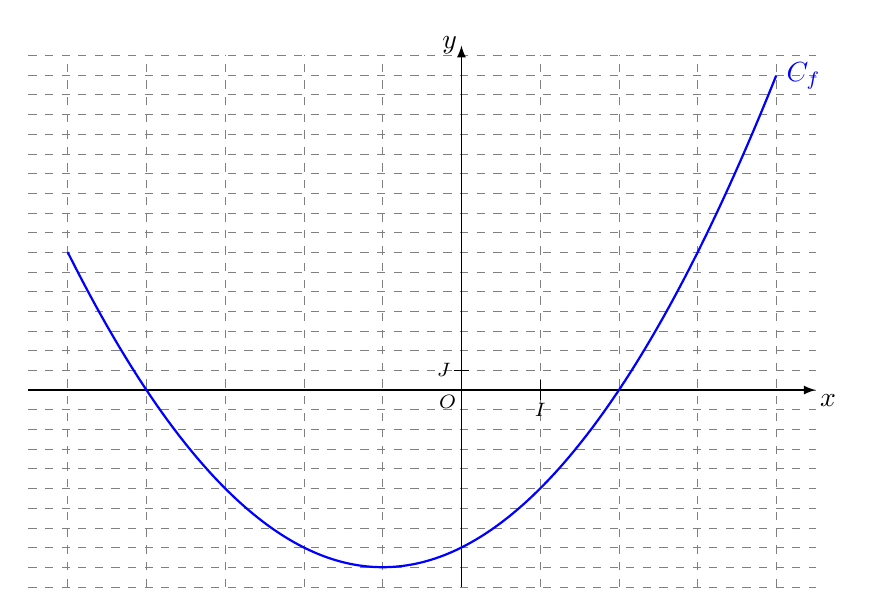
\begin{tikzpicture}[>=latex,yscale=0.25]
    \draw[help lines,dashed] (-5.5,-10) grid (4.5,17);
    \draw[line width=0.5pt,->] (-5.5,0) -- (4.5,0) node[below right=-2pt] {$x$};
    \draw[line width=0.5pt,->] (0,-10) -- (0,17.5) node[left=-2pt] {$y$};
    \draw (1,-0.5) -- (1,0.5); \draw (-0.1,1)--(0.1,1);
    \begin{scriptsize}
    \draw (0,0) node[below left=-1pt] {$O$};
    \draw (1,0) node[below=2pt] {$I$};
    \draw (0,1) node[left=1pt] {$J$};
    \end{scriptsize}
    \draw[blue,thick,domain=-5:4,samples=200]plot(\x,{(\x+1)^2 - 9}) node[right] {$\calig C_f$};
\end{tikzpicture}
\end{center}

\begin{enumerate}
    \item \textbf{Par lecture graphique :}
    \begin{enumerate}
        \item Donner l'intervalle de définition $\calig D_f$.
        \item Donner l'image de $-5$ par la fonction $f$.
        \item Déterminer $f(-2)$.
        \item Dire si le point $A(-3 \pv -5)$ appartient à $\calig C_f$.
        \item Déterminer, s'ils existent, les antécédents des nombres suivants : $16$ ; $0$ ; $-10$.
    \end{enumerate}
    \item \textbf{Par le calcul :} la fonction $f$ est définie pour tout $x \in \R$ par $f(x) = (x + 1)^2 - 9$.
    \begin{enumerate}
        \item Calculer $f(1)$.
        \item Calculer l'image de $\frac 74$ par la fonction $f$.
        \item Résoudre l'équation $f(x) = 0$.
        \item Calculer les antécédents du nombre $-8$.
        \item Déterminer par le calcul si le point $B\left(\frac12 \pv -6\right)$ appartient à la $\calig C_f$.
    \end{enumerate}
\end{enumerate}

\exo On considère la fonction $g$ définie pour tout $x \in \calig D_g$ par $g(x) = \sqrt{3x - 6}$.
\begin{enumerate}
    \item Résoudre l'inéquation $3x - 6 < 0$.
    \item Déterminer $\calig D_g$, ensemble de définition de $g$.
    \item Calculer $g(3)$. Peut-on calculer $g(1)$ ?
    \item Donner les antécédents des nombres $5$ et $-2$.
\end{enumerate}

\exo\medskip

\begin{minipage}{0.45\linewidth}
On donner l'algorithme suivant :
\begin{center}
\small
    \psframebox{
    \parbox{0.8\linewidth}{
        \textbf{Variables}\par
            \quad $x, a, b, c$ : nombres réels\par
        \textbf{Entrée}\par
            \quad Saisir $x$\par
        \textbf{Traitement}\par
            \quad Affecter à $a$ la valeur $x^2$\par
            \quad Affecter à $b$ la valeur $2x$ \par
            \quad Affecter à $c$ la valeur $a-b-3$\par
        \textbf{Sortie}\par
            \quad Afficher $c$
    }}
\end{center}
\end{minipage}
\begin{minipage}{0.53\linewidth}
\begin{enumerate}
    \item Quelle est la fonction $h$ définie par cet algorithme ?
    \item À l'aide de la calculatrice, écrire le tableau de valeurs de cette fonction entre $-2$ et $4$ avec une graduation de $0,5$.
    \item Représenter la fonction $h$ dans un repère orthonormé $\OIJ$ en choisissant \textbf{deux carreaux} comme unité.
\end{enumerate}
\end{minipage}
\end{document} 